\documentclass[letterpaper]{article}
\usepackage{aaai20}
\usepackage{times}
\usepackage{helvet}
\usepackage{courier}
\usepackage[hyphens]{url}
\usepackage{graphicx}
\usepackage{amsmath}
\urlstyle{rm}
\def\UrlFont{\rm}
\usepackage{graphicx}
\frenchspacing
\setlength{\pdfpagewidth}{8.5in}
\setlength{\pdfpageheight}{11in}
% Add additional packages here, but check
% the list of disallowed packages
% (including, but not limited to
% authblk, caption, CJK, float, fullpage, geometry,
% hyperref, layout, nameref, natbib, savetrees,
% setspace, titlesec, tocbibind, ulem)
% and illegal commands provided in the
% common formatting errors document
% included in the Author Kit before doing so.
%
% PDFINFO
% You are required to complete the following
% for pass-through to the PDF.
% No LaTeX commands of any kind may be
% entered. The parentheses and spaces
% are an integral part of the
% pdfinfo script and must not be removed.
%
\pdfinfo{
	/Title (Type Your Paper Title Here in Mixed Case)
	/Author (John Doe, Jane Doe)
	/Keywords (Input your keywords in this optional area)
}
%
% Section Numbers
% Uncomment if you want to use section numbers
% and change the 0 to a 1 or 2
% \setcounter{secnumdepth}{0}
% Title and Author Information Must Immediately Follow
% the pdfinfo within the preamble
%

\title{Learned Navigation Policies in the Absence of a Goal}
\author{Patrick Naughton, \ Tushar Kusnur, \ Ishani Chatterjee, \ and \ Maxim Likhachev\\
Address line\\
}


\begin{document}
	
	\maketitle
	
	\begin{abstract}
		Probabilistic planners have demonstrated promising results in dealing with robotic navigation under uncertainty \cite{ppcp}, for example, when parts of a map are unknown or the robot must navigate amongst other unpredictable agents. To compute trajectories, probabilistic planners rely on atomic actions which are strung together to form a path. Planners will often invoke a lower level controller to execute these actions. Existing work focuses on situations in which the humans in the scene move such that completion of the desired action is always feasible. Little attention has been paid to scenarios in which humans make reaching the goal waypoint impossible or prohibitively costly. Current methods may simply attempt to replan in these cases which can be too slow to avoid imminent collisions. Additionally, if the waypoint is unreachable or costly to reach, this approach may incur a higher cost than abandoning the waypoint and moving to a different location first before replanning. This paper presents a reinforcement learning based approach to developing \textit{failure controllers} for exactly these situations which direct the robot to an optimal failure location if its original goal waypoint becomes unreachable. We also present a method for determining when this controller should be employed by the robot that leverages calibrated estimates of the uncertainty of the robot in its next move. We refer to this element as a \textit{discriminator}. The combination of a failure controller with this discriminator allows the robot to determine when it is unable to reach its intended goal and to react to the situation accordingly, generating safer, more efficient trajectories.
	\end{abstract}
	
	\section{Introduction}
		Pedestrian crowds present a challenging navigation environment for a mobile robot. The robot must comply with latent social rules governing its trajectory while simultaneously reaching its goal in a reasonable amount of time. As robots move into closer contact with humans, advanced methods for navigation in crowds will gain increased importance. Probabilistic planners, which make navigation plans in the belief space, show potential to make headway in this problem and have demonstrated success dealing with uncertainty like that experienced navigating in a crowd. To form their plans, these planners rely on smaller atomic actions which are strung together to form an overall trajectory. Some of these actions are learned by presenting the robot with its starting pose and a waypoint pose and running simulations with pedestrians or other agents \cite{crowdawarerl}. In general, these controllers guiding each action deal with unexpected situations in which their original trajectory to their waypoint becomes infeasible by simply replanning or stopping altogether. Replanning in some cases may take too long to avoid an imminent collision. Additionally, when the waypoint becomes completely unreachable, replanning or stopping may result in a more costly trajectory than simply abandoning it and seeking a safe location from which the higher level planner can generate a new trajectory to the overall goal. We address this issue by segmenting the robot's navigation policy when a particular action is invoked. Specifically, the robot defaults to executing a \textit{success controller} which attempts to guide the robot around pedestrians to its short-term goal. A \textit{discriminator} determines if and when the robot should switch to the \textit{failure controller} that corresponds to this success controller. The failure controller provides a navigation policy for the robot to follow in cases where the robot's waypoint is unreachable and the success controller may command an overly aggressive trajectory.
		
		Previous work has made substantial headway in creating success controllers using imitation and reinforcement learning techniques \cite{tai2018socially}, \cite{crowdawarerl}. This work facilitates combining learning with planning for long term crowd navigation by providing a reinforcement learning based failure controller and a discriminator to determine when to execute this controller. Specifically, this paper assumes that an existing probabilistic planner uses a set of motion primitives and controllers to create navigation plans. The set of controllers includes some to execute complex behaviors that interact with pedestrians. Each of these controllers has some probability of success which is associated with one goal and trajectory, and some probability of failure which is associated with a different trajectory. Success cannot be guaranteed for the controllers because the surrounding humans may interact with the robot or each other in unexpected ways. Note that the failure controller's objective differs from that of a traditional navigation planner in that the failure controller is not given an explicit goal; rather, it attempts to extract the optimal goal and trajectory from its environment. 
		
		The main contributions of this work are:
		\begin{enumerate}
			\item A reinforcement learning based controller for commanding robot trajectories in cases of failure.
			\item A framework for implementing a discriminator that judges whether or not to begin executing the failure controller. This discriminator assumes that the success controller is implemented as a neural network.
		\end{enumerate}
		The design philosophy taken by this approach separates controllers for individual actions from the long term planner. This means the results presented here could easily be adapted to work with any planner.
		
		The remainder of this paper is organized as follows. Section \ref{sec:background} discusses background information on the problem presented here including related work and a formalized statement of the problem. Section \ref{sec:approach} lays out the approach taken to construct and train both the failure controller and the predictor. Section \ref{sec:experiments} describes the experiments carried out to test the discriminator and failure controller. Section \ref{sec:results} gives the results of simulation experiments. Finally, Section \ref{sec:conclusion} draws conclusions from these experiments and suggests future research directions.
		
		The complete code of our approach is available here: \texttt{\url{https://github.com/patricknaughton01/LearnController}}.
	\section{Background}\label{sec:background}
		This section provides the necessary background information to contextualize the problem examined here. This includes summarizing the related work in this area and formalizing the precise problem statement we seek to solve.
		 
		\subsection{Related Work}
			Several methods use explicit models of human behavior to achieve smooth, predictable robot navigation among pedestrians. Trautman et al. model the interaction between the robot and pedestrians as an extension of an interactive Gaussian process that accommodates multiple goals \cite{caseforcoop}. The social forces model \cite{sfm} treats humans and the robot in question as masses subject to Newtonian dynamics and applies fictitious forces to them to predict and plan trajectories. It recomputes these forces and their effects on robot motion at each time step to determine how the robot should move. These techniques however rely on hand-crafted models of human behavior to achieve their results and handle unexpected or uncooperative human actions by simply replanning using the same model. The social forces model in particular does not demonstrate robust navigation plans and will sometimes exhibit oscillatory behavior in more crowded or narrow areas \cite{sfm}. 
			
			Another approach uses inverse reinforcement learning to learn latent, possibly stochastic social rules humans observe when navigating in crowds \cite{socialirl}. This method uses example trajectories recorded from humans or gathered from teleoperated runs. This approach however is extremely unlikely to observe failed trajectories where a human attempts to execute some navigation plan and is forced to completely abort their initial goal. If a human attempts to overtake someone else, for example, they have many contingency options in the case where the other person is either intentionally or unintentionally uncooperative. For example, they could use verbal communication or body language to more explicitly communicate their intentions, options which are not available to many mobile robots. For this reason, inverse reinforcement learning will likely be unable to formulate a useful model for navigation when situations such as these occur.
			
			Advances in deep reinforcement learning have led many to apply it to this problem. After demonstrating its capability to match and in some cases exceed human performance in a variety of video games \cite{atarirl}, much research has focused on applying it to different domains. It has successfully been applied to the social robot navigation problem using a variety of different models \cite{sociallyawarerl}, \cite{crowdawarerl}. Reinforcement learning is particularly suited to this application as noted in \cite{sociallyawarerl} because it is extremely difficult to specify what the optimal action for a robot to take is but it is much easier to alert the robot when it takes a socially unacceptable or unsafe action. Previous work has focused on using reinforcement learning to develop policies that generate optimal (in terms of time) paths to a robot's goal in the presence of humans or other autonomous agents. These policies however generally assume the goal is reachable and do not make contingency plans if that assumption turns out to be incorrect. Additionally, the agent is explicitly given a goal to reach by the experimenters; we wish to navigate in the case of failure at which point there is no obvious goal.
			
			The above methods all have proven successful in developing success controllers. However, they either deal with failure at execution time by simply replanning or do not consider failure to reach the goal at all. We depart from this paradigm by designing a controller specifically targeted at producing trajectories when the robot's original goal is no longer reachable.
		
		\subsection{Problem Statement}
			The problem statement is two-fold. First, a failure controller that can direct the robot in cases where it has no navigation goal is sought. This is in the form of a policy selecting one of the robot's possible actions conditioned on the its current state. Second, we wish to determine at each time step whether or not the robot should start executing its failure controller for a given scene. This should occur if and only if the robot determines that its original navigation goal is infeasible (or is likely to be infeasible).
			
			\subsubsection{Failure Controller}
				Consider a robot using a probabilistic planner to navigate in a pedestrian environment. The environment contains both static and dynamic obstacles in the form of humans and other objects. This robot has a set $M$ of motion primitives which it can use to perform simple movements. The robot also has a set $C$ of controllers which it can execute to perform more complex behaviors that may require cooperation from humans. Because these controllers have some probability of failing, the robot needs a contingency plan to follow that will return it to a safe location. 
				
				This paper demonstrates our framework by applying it to a \textit{barge-in} controller. This controller addresses a situation in which humans block a narrow corridor and the robot wishes to move past them. Ideally, the robot would drive towards the group of people who would then part enough for the robot to reach its goal. However, if the people do not move---for example, if they do not notice the robot or they cannot infer its intention to move past them---the robot needs a contingency plan that results in safe behavior and brings the robot back to a location from which it can replan.
				
				We model the problem of finding the optimal failure policy as solving a Markov Decision Process $\langle\mathcal{S}, \mathcal{A}, \mathcal{R}, \mathcal{P}, \gamma\rangle$ with an infinite set of states $\mathcal{S}$, a finite set of actions $\mathcal{A}$, state transition matrix $\mathcal{P}(s_t, a_t, s_{t+1})$, reward function $\mathcal{R}(s_t, a_t, s_{t+1})$ and discount factor $\gamma \in (0, 1)$ \cite{suttonandbarto}. The robot seeks an optimal policy $\pi^*(a_t \mid s_t)=P(a_t \mid s_t)$ where optimal indicates that the policy maximizes the overall expected discounted reward the robot receives (referred to as the "return" of the policy) from the current time step $t$ onwards:
				
				\begin{equation}\label{eq:discountedreturn}
					\sum_{k=0}^{\infty}E[\gamma^k \mathcal{R}(s_{t+k}, a_{t+k}, s_{t+k+1})]
				\end{equation}
				
				To aid in finding this policy, we define a $Q_{\pi}(a_t, s_t)$ function which estimates the return of executing action $a_t$ from state $s_t$ and following policy $\pi$ from that point onwards:
				
				\begin{equation}\label{eq:q}
					Q_{\pi}(a_t, s_t) = 
					\sum_{k=0}^{\infty}E[\gamma^k \mathcal{R}(s_{t+k}, \pi(a_{t+k} \mid s_{t+k}), s_{t+k+1})]
				\end{equation}
				\begin{align}
					\begin{split}\label{eq:bellmanexpect}
						Q_{\pi}(a_t, s_t) =& 
						\sum_{s'\in \mathcal{S}}\mathcal{P}(s_t, a_t, s')[\mathcal{R}(s_t, a_t, s') \\
						&+ \gamma \sum_{a'\in \mathcal{A}}\pi(a'\mid s')Q_{\pi}(a', s')]
					\end{split}
				\end{align}
				
				Assuming $\pi$ is greedy, we can rewrite\footnote{This rewrite also makes use of the fact that the ground-truth next state is an unbiased estimator of the expected next state.}
				
				\begin{equation}\label{eq:simplebellmanexpect}
					Q_{\pi}(a_t, s_t) = \mathcal{R}(s_t, a_t, s_{t+1}) + \gamma max_a Q_{\pi}(a, s_{t+1})
				\end{equation}
				
				We denote the $Q$ function of the optimal policy as $Q^*$. $Q^*$ gives a convenient way to determine the optimal action for any state given that the action space is finite and small because we can simply find the action with the largest $Q^*$ value and execute it.
				
			\subsubsection{Discriminator}
				At each time step, the discriminator indicates whether or not the robot should stop executing its current controller and transition to the corresponding contingency plan (failure controller). Once the robot has made this transition it cannot return to its original controller until the failure controller has finished its execution and the robot has determined it is safe to replan. Therefore, we wish to develop a discriminating criterion that is met if and only if the robot would truly be better off (would execute a safer or more efficient trajectory) if it switches to its failure controller.
				
				In this paper, we specifically focus on navigation controllers represented by a neural network. Intuitively, we wish to know whether or not this network is confident that it can reach its intended goal. We judge this confidence by measuring the uncertainty of the network in its prediction of the next step for the robot to take and make the discriminator a function of this uncertainty. More precisely, our discriminator is a binary classifier which takes as input the success controller's total predictive uncertainty at each time step and outputs whether or not the robot should switch to its failure controller.
	\section{Approach}\label{sec:approach}
			Both the success and failure controllers are represented as neural networks. 
			
			\subsection{Failure Controller}
				\subsubsection{State Representation}
				Because the MDP we have described has infinitely many states, it is impossible to store a $Q$ value for each state-action pair explicitly. We base our state characterization on that presented in \cite{crowdawarerl} with slight modifications because of our controller's lack of a goal. An initial matrix is constructed with the same number of rows as there are agents and obstacles in the scene (including the robot). Each row of the matrix takes the form $(s_\text{pref}, h, r, v_x, v_y, p'_x, p'_y, v'_x, v'_y, r', d, r_\text{sum})$ where 
				\begin{itemize}
					\item $s_\text{pref}$ is the preferred speed of the robot.
					\item $h$ is the heading of the robot w.r.t. the global coordinate frame.
					\item $r$ is the radius of the robot.
					\item $v_x$ and $v_y$ are the x and y velocities of the robot w.r.t. the robot's coordinate frame.
					\item $p'_x$ and $p'_y$ are the x and y coordinates of the other agent w.r.t. the robot's coordinate frame.
					\item $v'_x$ and $v'_y$ are the x and y velocities of the other agent w.r.t. the robot's coordinate frame (note, this is not relative to the robot's velocity, just relative to its rotation).
					\item $r'$ is the radius of the other agent.
					\item $d$ is the Euclidean distance between the robot and the other agent.
					\item $r_\text{sum}$ is the sum of the radii of the robot and the other agent.
				\end{itemize}
				The first five components of each row are referred to as the robot's \verb|self_state| because they pertain specifically to the robot.
				
				This is augmented by a series of occupancy maps, one for each human and obstacle in the scene and one for the robot itself. Each occupancy map is centered on and aligned with its respective agent and their heading and is discretized into a number of squares. Each square indicates in a binary fashion whether or not it contains an object. Each square also contains the average velocity of all the objects within that square (simply set to 0 if the square is unoccupied). In our case, each occupancy map is discretized into 16 (4x4) 1 unit squares. This collection of occupancy maps and information about the robot's dynamics form the robot's \textit{state}. Note that the dimensions of the state matrix will vary depending on the number of humans and obstacles in the scene.
				
				For the purposes of computing the position, velocity, and heading of a given obstacle we simply consider the point on the obstacle which is closest to the robot. Any obstacle will always have a velocity of 0 and a heading along the robot's x-axis.
				\subsubsection{Q Function}
				There are 35 different available actions in any given state. One is to do nothing (remain in the same location). There are then 16 directions the robot can move w.r.t. its heading which are evenly spaced from $0$ to $2\pi$ (we assume a holonomic robot) and the robot can travel at either half or full speed in each of these directions. Finally, the robot can also rotate in either direction by a small amount. We represent $Q_\pi$ using a deep neural network whose architecture is based on that presented in \cite{crowdawarerl} which showed that it could generate satisfactory goal-oriented trajectories navigating amongst humans. The state of the robot is first given to a Multi-Layer Perceptron (MLP). This output is processed by two additional MLPs, one of which computes weights and one of which computes features. The weight MLP also receives the average of the input MLP's outputs across the different rows of the state matrix. The weights returned from this MLP are then passed through a softmax layer. The dot product of the features and softmaxed weights is then computed which yields a constant size vector (independent of the number of agents and obstacles in the scene). This result, along with the robot's \verb|self_state| are then fed into a layer of LSTM cells. The outputs of these cells are processed by a final MLP which generates $Q$ values for each of the 35 different possible actions simultaneously. 
				
				The different components of the overall network have the following dimensions: [60, 80], [80, 120], [160, 64, 31, 1], [86, 256], [256, 128, 64, 35] for the input MLP, feature MLP, weight MLP, LSTM, and output MLP respectively. 
				
				\begin{figure}
					\centering
					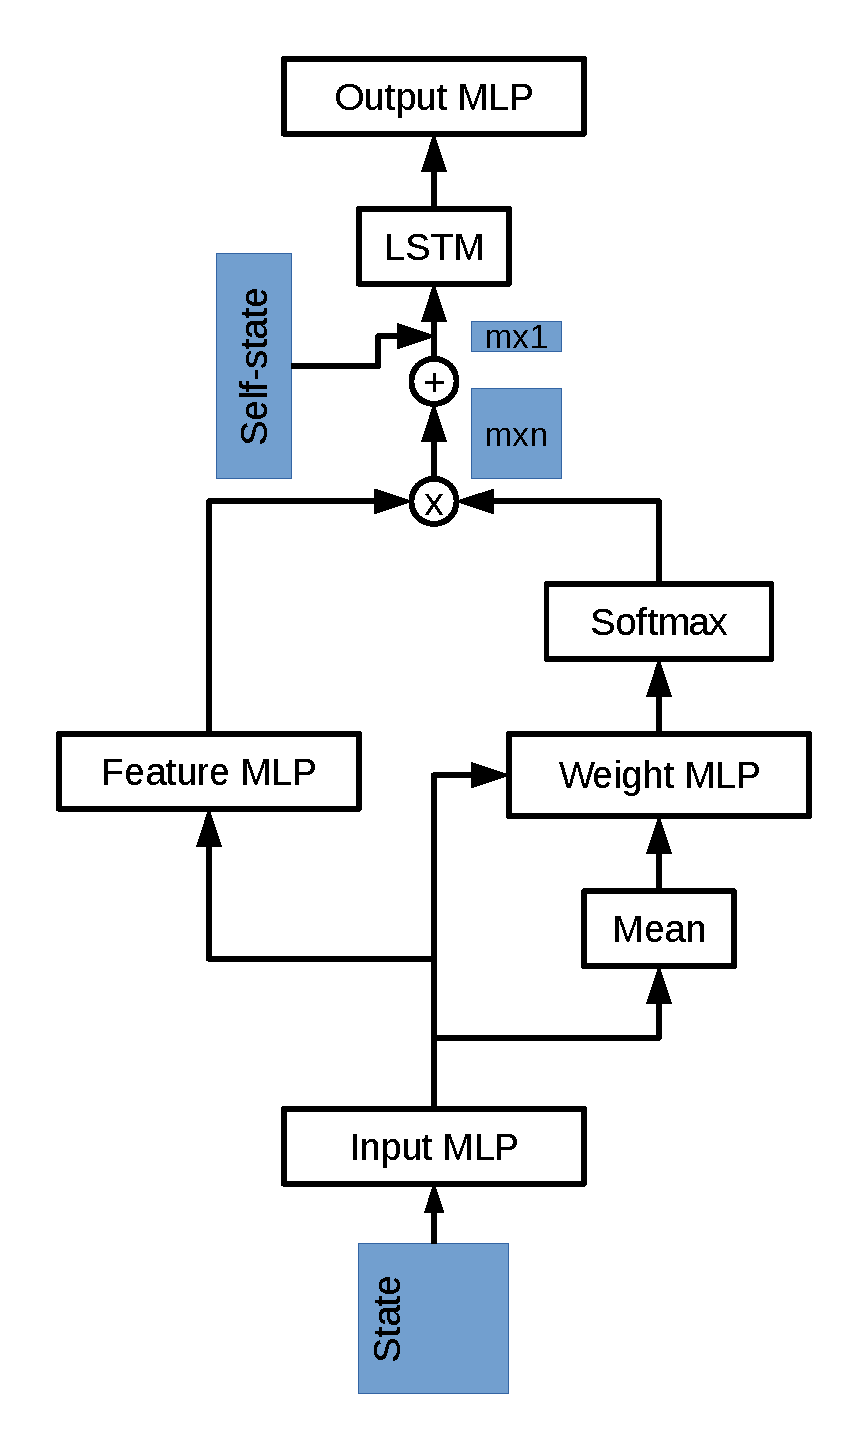
\includegraphics[height=\linewidth, angle=270, origin=c]{model_arch}
					\caption{Architecture of our network for learning the $Q_\pi$ function. Since the number of humans in the scene could vary, the state input is not a constant size. The weighted features get summed across each agent to form a constant size vector before being given to the LSTM.}
					\label{fig:model_arch}
				\end{figure}
				\subsubsection{Reward function}
				The reward function $\mathcal{R}(s_t, a_t)$ at each time step is computed in three parts: $\mathcal{R}_{collision}$, $\mathcal{R}_{movement}$, and $\mathcal{R}_{smoothness}$ for collision, movement, and smoothness rewards respectively. The components are defined in the following way:
				\[
				\mathcal{R}_{collision} = \begin{cases}
				-1      &   d < 0\\
				-0.25   &   0 \leq d < 0.2\\
				0       &   else
				\end{cases}
				\]
				Here, $d$ denotes the distance between the robot and an obstacle or another agent. Note that this reward is applied individually with respect to each human and obstacle in the scene so if the robot is colliding with two humans simultaneously it will receive a reward of $-2$. When the robot occupies the second region ($0\leq d < 0.2$) we refer to this as an \textit{intrusion} and call the upper bound of $0.2$ the \textit{intrusion threshold}. This component disincentivizes colliding with humans and obstacles. It is based on the reward function used in \cite{crowdawarerl}. Additionally, for each human or obstacle the robot is forecasted to collide with or intrude into (based on current velocities) the robot receives a reward of $-0.05$ (for predicted collisions) and $-0.0125$ (for predicted intrusions). This was done to make the reward function smoother.
				\[
				\mathcal{R}_{movement} = \begin{cases}
				0       &   a_t = 0 \quad(remain\;still)\\
				-0.01   &   else
				\end{cases}
				\]
				This component is meant to very slightly punish moving so that areas farther from the robot's initial location are less desirable. It was added because, all other things equal, areas closer to the robot's initial position are preferred because they can be reached more quickly.
				\[
				\mathcal{R}_{smoothness} = \begin{cases}
				0       &   a_t = a_{t-1} \vee a_{t-1} = 0\\
				-0.01   &   else
				\end{cases}
				\]
				The smoothness component of the reward incentivizes using the same action repeatedly so that the robot prefers smooth trajectories. These trajectories are qualitatively more predictable for humans which makes them easier to navigate around and result in plans which are generally easier to execute.
				
				The total reward at each time step is simply the sum of these three components.
				\subsubsection{Training} 
				To simulate the robot moving about in a pedestrian environment the RVO2 library as well as its Python wrapper were used \cite{rvo2}, \cite{pyrvo2}. This library provides a convenient way to simulate an environment with multiple autonomous agents and obstacles. It uses the Optimal Reciprocal Collision Avoidance (ORCA) \cite{orca} algorithm to generate safe velocity vectors for each agent to follow to reach a predefined goal.
				
				For the barge-in scenario, each training episode starts with the robot right behind a group of humans blocking a narrow passage as though it had approached attempting to move past them. The width of the corridor, number and size of the humans, and the initial position and size of the robot are all initialized with small random perturbations. Each human sets a goal at a random location inside the corridor which would force the robot to abort its normal plan. The robot then begins executing actions according to an epsilon-greedy strategy, choosing a random action with probability $\epsilon \in [0, 1]$ and otherwise choosing the action with maximum estimated $Q$ value. When the robot selects an action, this only sets its preferred velocity. The underlying simulator may modify the actual velocity it commands if an imminent collision is detected. 
				
				We use the deep Q-learning algorithm with experience replay to train our Q-network \cite{dqn}. Two copies of the Q-network are stored, one called the \verb|policy_model| and one called the \verb|target_model|. The simulated robot follows an epsilon-greedy policy and records a tuple containing the state, action, reward received, and next state at each time step in a memory buffer. It then samples a batch of these tuples and updates the \verb|policy_model|. Pseudocode for this algorithm is presented in Algorithm \ref{algo:dqn}.
				
				The \verb|target_model| and \verb|policy_model| were implemented using PyTorch. An Adam optimizer with a learning rate of 0.001 was used to make updates to the \verb|policy_model|'s weights and each MLP had a dropout probability of $0.1$. $\epsilon$ started at $1.0$ and linearly annealed to $0.1$ over $250000$ time steps. $\gamma$ was set to $0.9$. Each episode consisted of $100$ time steps (corresponding to approximately 10 seconds). The mean squared error loss function was used to compute the loss between the \verb|policy_model|'s predictions and their targets.
			
			\subsection{Discriminator}
				To determine whether or not the robot is likely to succeed in a given scene, we determine the uncertainty of the success controller and compare it to a threshold. If it ever exceeds a precomputed threshold (specific to each controller), then the robot transitions to its failure controller and continues executing it until it reaches its timeout. For particularly unstable scenes where the uncertainty fluctuates greatly between time steps, it may be appropriate to examine the rolling average of the uncertainties rather than the value itself at each time step. 
				
				In order to compute this threshold, we create a training set of success examples for a given scene. This training set consists of many (1000) trial runs in which the robot successfully reaches its goal in a given scene, stored as time series data of the locations and velocities of the robot and each human. 
				
				The success controller network has the same architecture as that of the failure controller, except it only has five outputs instead of $35$. These outputs represent the expected next position of the robot, $(p_x, p_y)$, the logarithm of the standard deviation of this prediction $(log\sigma_x, log\sigma_y)$, and the inverse hyperbolic tangent of the correlation between the $x$ and $y$ prediction $(tanh^{-1}(\rho))$. This network is trained using a negative two-dimensional Gaussian log-likelihood loss where the target at each time step is the ground truth robot position at the next time step. This network is trained with a high dropout probability of $0.4$ for $300$ epochs. At testing time, to determine the uncertainty of the network's prediction, we add its data uncertainty to its model uncertainty. To compute these values, we simply run the robot's observed state through the network some number of times ($20$ in our specific case) to find the average standard deviation in the $x$ and $y$ directions reported by the network (data uncertainty) as well as the standard deviations of the target positions reported by the network for both the $x$ and $y$ directions (model uncertainty). These two values are summed to find the total uncertainty in each direction \cite{uncertaintyindeeplearning}. To find the square of the overall magnitude of this uncertainty we sum the squares of these individual components.
				
				At testing time, we simply see if this total uncertainty magnitude exceeds a precomputed threshold. To find this threshold, we simulated the success controller in $100$ cases similar to the training data set that allowed the robot to reach its goal, and $100$ cases in which the robot could not reach its goal due to human movement it the scene. Each trial ran for $100$ time steps. We then examined the maximum uncertainty realized in each of these trials by the success controller and chose a threshold that minimized the total number of erroneous categorizations (the sum of the number of familiar trials with higher uncertainty and unfamiliar trials with lower uncertainty). This threshold is then set for this specific success controller.
			
	\section{Experiments}\label{sec:experiments}
		To test the effectiveness of our approach we ran three different types of trials for a \textit{barge-in} controller (working on some of them, as well as overtake). This controller applies to a scene in which a group of humans are standing at the end of a hallway and the robot would like to barge past them to reach a goal on the opposite side. In a successful execution of this controller, the humans will move out of the way for the robot to pass through. In an unsuccessful execution, the humans may remain stationary or may even move into the corridor, preventing the robot from passing. 
		
		We test first on an unfamiliar scene in which the humans move into the corridor the robot occupies. In one set of trials, we enable the discriminator and failure controller so that the robot will respond to the novel scene by transitioning to its contingency plan once it realizes that its original goal is infeasible (specifically, once it is suitably uncertain that it will reach its intended goal). If the robot's uncertainty never reaches this threshold after $100$ time steps, the trial is simply ended. The failure controller was run for $100$ time steps before being cut off. 
		
		(I haven't done this experiment yet but it should be quick, hopefully)In the next set of trials, we deactivated the discriminator such that the success controller would run until it was cut off after $100$ time steps. The robot then follows this policy and ignores its uncertainty throughout the trial.
		
		Finally, in the last set of trials we placed the robot in a familiar scene with the failure controller and discriminator activated. This was done to ensure that the robot does not aggressively trigger the failure controller: it should only be used when the robot is truly uncertain about its ability to reach the goal. These trials serve to verify that the uncertainty threshold is high enough: the robot will continue following its success controller as long as it is reasonably certain it can reach its goal. 
		
	\section{Results}\label{sec:results}
		After carrying out $100$ of each type of trial, the overall paths produced in each run were rated according to:
		\begin{itemize}
			\item Path length: The total distance traveled by the robot. In general we would like the robot to move less when possible (find the shortest path when executing a success controller and minimize backwards progress when executing the failure controller).
			\item Angular distance: The changes in heading the robot underwent. This is used to approximate the smoothness of the robot's path.
			\item Collisions: The sum of the number of people the robot is in collision with in each time step. We place the highest priority on minimizing this value.
			\item Intrusions: The sum of the number of people the robot intrudes on in each time step. An intrusion is defined as the robot being within $0.2m$ of a person. All other things equal, we would like to decrease the number of intrusions, but some number of them are acceptable if they are necessary to reach the goal.
		\end{itemize}
		
		(Insert table of results)
	
	\section{Conclusion}\label{sec:conclusion}
	
	% References and End of Paper
	% These lines must be placed at the end of your paper
	\bibliography{ref}
	\bibliographystyle{aaai}
	
\end{document}